  \documentclass{article}


\usepackage{arxiv}

\usepackage[utf8]{inputenc} % allow utf-8 input
\usepackage[T1]{fontenc}    % use 8-bit T1 fonts
\usepackage{hyperref}       % hyperlinks
\usepackage{url}            % simple URL typesetting
\usepackage{booktabs}       % professional-quality tables
\usepackage{amsfonts}       % blackboard math symbols
\usepackage{nicefrac}       % compact symbols for 1/2, etc.
\usepackage{microtype}      % microtypography
\usepackage{lipsum}
\usepackage{graphicx}
\usepackage{amsmath}
\newtheorem{definition}{Definition}

\usepackage{algorithm}
\usepackage{algpseudocode}
\DeclareMathOperator*{\E}{\mathbb{E}}
\newcommand{\Pprob}{\text{I\kern-0.15em P}}
\DeclareMathOperator*{\argmax}{arg\,max}

\usepackage{booktabs}
\usepackage{longtable}
\usepackage{makecell}

\usepackage{makecell}
\renewcommand\theadfont{\bfseries}

\usepackage{caption}
\usepackage{subcaption}
\newcommand{\norm}[1]{\left\lVert#1\right\rVert}



\graphicspath{ {./images/} }

\title{AML in depth study: Reinforcement learning}


\author{
 Gianluca Giudice\\
  University of Milano-Bicocca\\
  \texttt{g.giudice2@campus.unimib.it} \\
}

\begin{document}
\maketitle
\begin{abstract}
The aim of reinforcement learning is to build an agent, or decision maker, that learn to achive a goal by interacting with the enviroment. This type of learning is performed through a sequence of rewards and punishment which depends on the decisions made by the agent. In reinforcement learning the agent aims to maximise the cumulative reward. In this work I'll give an introduction to reinforcement learning, starting from the fundamental aspects until the latest deep reinforcement learning techniques. As an example of deep reinfroceemnt learning I'll present and explain AlphaGo zero \cite{silver2017mastering}, one of the most famous application of reinforcement learning, where David Silver et. al managed to build an agent without human knowledge able to achive superhuman performance in the game of Go. At the end of this work, based ont AlphaGo zero, I'll develop an algorithm to master the game of connect4 without human knowledge.
\end{abstract}

\section{Introduction}

Reinforcement learning is a computational approach to understanding and automating goal-directed learning and decision making. In this framework, learning is inteded as mapping situations to actions so as to maximize a numerical reward signal. The learner is not told which actions to take, but instead must discover which actions yield the most reward by trying them thorugh interactions with the environment. In the most interesting and challenging cases, actions may affect not only the immediate reward but also the next situation and, through that, all subsequent rewards. Trial-error and delayed reward  are the two most important distinguishing features of reinforcement learning \cite{10.5555/3312046}.

Markov decision processes are used in the reinforcement learning framework to formally describe the environment. A learning agent must be able to sense the state of its environment and must be able to take actions that affect the state in order to achive a goal. Markov decision processes include a sense of sensation, action and goal, the essential features of the problem which represents a sense of cause and effect. Any method that is well suited to solving such problems is considered to be a reinforcement learning method.

In many complex domains, reinforcement learning is the only feasible way to train a program to perform at high levels. For example, in game playing, it is very hard for a human to provide accurate and consistent evaluations of large numbers of positions, which would be needed to train an evaluation function directly from examples. Instead, the program can be told when it has won or lost, and it can use this information to learn an evaluation function that gives reasonably accurate estimates of the probability of winning from any given position. Similarly, it is extremely difficult to program an agent to fly a helicopter; yet given appropriate negative rewards for crashing, wobbling, or deviating from a set course, an agent can learn to fly by itself \cite{russell2016artificial}.


\section{Key Concepts in Reinforcement Learning}

The main characters of RL are the agent and the environment. The environment is the world that the agent lives in and interacts with. At each time $t$, the agent receives the current state $s_t$ and reward $r_t$. It then chooses an action $a_t$ from the set of available actions, which is subsequently sent to the environment. The environment moves to a new state $s_{t+1}$ and the reward $r_{t+1}$ associated with the transition $(s_{t},a_{t},s_{t+1})$ is determined.

\begin{figure}
	\centering
	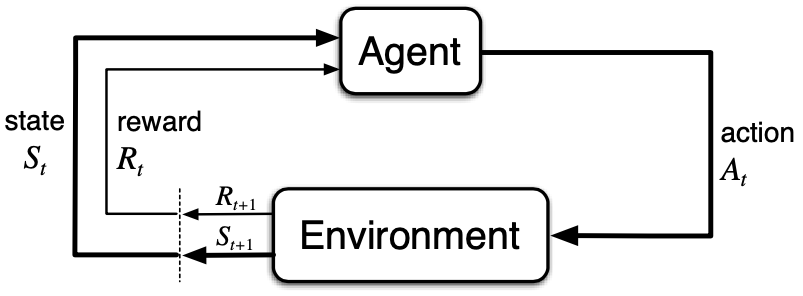
\includegraphics[width=8cm]{rl-loop.png}
	\caption{Typical RL scenario. \cite{10.5555/3312046}}
	\label{fig:rl-loop}
\end{figure}

To talk more specifically what RL is about, it's important to go through these key concepts \cite{SpinningUp2018}: 

\begin{itemize}
	\item States and observations
	\item Action spaces
	\item Policies
	\item Reward and return
	\item RL optimization problem
	\item Value functions
\end{itemize}


\subsection{States and observations}
A \textbf{state} $s$ is a complete description of the state of the world. There is no information about the world which is hidden from the state. An \textbf{observation} $o$ is a partial description of a state, which may omit information. When the agent is able to observe the complete state of the environment, it is fully observed. When the agent can only see a partial observation, the environment is partially observed.

Markov decision processes (Markov Reward Processes plus actions), are a classical formalization of sequential decision making, where actions influence not just immediate rewards, but also subsequent situations, or states, and through those future rewards. To this reason MDPs are a mathematical way to describe the reinforcement learning problems. 

\begin{definition}
	A \textbf{MDP} is a tuple $(S,A, P, R, \gamma)$, where:
	\begin{itemize}
		\item $S$ is a (finite) set of Markov states $s \in S$
		\item $A$ is a (finite) set of actions $a \in A$
		\item $P$ is dynamics/transition model for each action, that specifies
		$$P(s_{t+1} =s'|s_t =s,a_t =a)$$
		\item $R$ is a reward function
		$$R(s_t =s,a_t =a)=\E[r_t|s_t =s,a_t =a]$$
		\item $\gamma$ is a discount factor $\gamma \in [0,1]$
	\end{itemize}
\end{definition}


\subsection{Action spaces}
Different environments allow different kinds of actions. The set of all valid actions in a given environment is called the \textbf{action space}. Some environments, like Atari and Go, have \textbf{discrete action spaces}, where only a finite number of moves are available to the agent. Other environments, like where the agent controls a robot in a physical world, have continuous action spaces. In continuous spaces, actions are real-valued vectors.

\subsection{Policies}
A \textbf{policy} defines the learning agent’s way of behaving at a given time, it's a mapping from perceived states of the environment (i.e. observations) to actions to be taken when in those states. A policy fully defines the behaviour of an agent:

\begin{definition}
	 A \textbf{policy} $\pi$ is a distribution over actions given states
	
	\begin{equation}
	\pi(a | s) = \Pprob[A_t=a|S_t=s]
	\end{equation}

\end{definition}

The MDP and agent's policy together give rise to a \textbf{trajectory} $\tau$, which is a sequence of states and actions in the world:
$$\tau = (s_0, a_0, r_0, s_1, a_1, r_1...)$$


\subsection{Reward and return}
The reward function $R$ depends on the current state of the world and action just taken:

$$r_t = R(s_t, a_t)$$

The agent aim to maximize the cumulative reward over a trajectory. The number of time steps in the trajectory is the \textbf{horizon}, denoted by $H$, and can be infinite. The sum of all rewards obtained by the agent is discounted by how far off in the future they’re obtained. The discount factor is $\gamma \in [0,1]$.

\begin{equation}
R(\tau) = \sum_{t=0}^{H-1} \gamma^t r_t
\end{equation}

\subsection{RL optimization problem}
The goal in RL is to \textbf{maximize the expected return} when an agent acts according to a policy. The policy influences the probability distribution over trajectories. The probability of a $T$-step trajectory is:

\begin{equation}
P(\tau|\pi) = \rho_0 (s_0) \prod_{t=0}^{T-1} P(s_{t+1} | s_t, a_t) \pi(a_t | s_t)
\end{equation}


The expected return, denoted by $J(\pi)$, is then:

\begin{equation}
J(\pi) = \E_{\tau\sim \pi}{[R(\tau)]}
\label{eq:loss}
\end{equation}

The central optimization problem in RL can then be expressed by
\begin{equation}
\pi^* = \arg \max_{\pi} J(\pi)
\label{eq:max_loss}
\end{equation}

with $\pi^*$ being the optimal policy.


\subsection{Value functions}
It's very important to point out the expected return by starting in a specific state or state-action pair. This is crucial since they are used in almost every RL algorithm.

There are two main functions \cite{silver2015}:


\begin{enumerate}
	\item The \textbf{State-Value Function} of a policy.
	
	\item The \textbf{Action-Value Function} of a policy.
	
\end{enumerate}

	
\begin{definition}
	The \textbf{State-Value Function} of a policy, $V^{\pi}(s)$ is the expected return by starting in state $s$ and always acting according to policy $\pi$:
	\begin{equation}
		V^{\pi}(s) = \E_{\tau \sim \pi} [R(\tau)| s_0 = s]
	\end{equation}
\end{definition}

\begin{definition}
	The \textbf{Action-Value Function} of a policy, $Q^{\pi}(s,a)$ is the expected return by starting in state $s$ and taking an arbitrary action $a$ (which may not have come from the policy), and then forever after acting according to the policy $\pi$:
	\begin{equation}
			Q^{\pi}(s,a) = \E_{\tau \sim \pi}[R(\tau)| s_0 = s, a_0 = a]	
	\end{equation}
	
\end{definition}

Starting form these definitions it's possible to introduce two other key functions:

\begin{enumerate}
	\item The \textbf{Optimal State-Value Function}.
	\item The \textbf{Optimal Action-Value Function}.
\end{enumerate}

The state value function and action value function are connected by the following relationship:

\begin{equation}
V^\pi(s) = \E_{a \sim \tau}[Q^\pi (s,a)]
\end{equation}

\subsection{Optimal value function and optimal policy }
Value functions define a partial ordering over policies. A policy $\pi$ is defined to be better than or equal to a policy $\pi'$ if its expected return is greater than or equal to that of $\pi'$ for all states. In other words, $\pi \geq \pi'$ if and only if $v_\pi(s) \geq v_{\pi'}(s)$ for all $s \in S$. There is always at least one policy that is better than or equal to all other policies. This is an optimal policy and it's denoted by $\pi*$.

\begin{definition}
	The \textbf{Optimal State-Value Function}, $V^*(s)$ is the expected return by starting in state $s$ and always acting according to the \textit{optimal} policy in the environment:
	
	\begin{equation}
		V^{*}(s) = \max_\pi \E_{\tau \sim \pi} [R(\tau)| s_0 = s] = \max_\pi V^\pi(s)
	\end{equation}
\end{definition}

\begin{definition}
	The \textbf{Optimal Action-Value Function}, $Q^*(s,a)$ is the expected return by starting in state $s$, taking an arbitrary action $a$, and then forever after acting according to the \textit{optimal} policy in the environment:
	
	\begin{equation}
	Q^*(s,a) = \max_{\pi} \E_{\tau \sim \pi}{[R(\tau)| s_0 = s, a_0 = a]} = \max_\pi Q^\pi(s,a)
	\end{equation}
	
\end{definition}
There is an important connection between the optimal action-value function $Q^*(s,a)$ and the action selected by the optimal policy.

By definition, $Q^*(s,a)$ gives the expected return for starting in state $s$, taking (arbitrary) action $a$, and then acting according to the optimal policy forever after. As a result, by having $Q^*(s,a)$, it's possible to directly obtain the optimal action $a^*(s)$:

\begin{equation}
a^*(s) = \argmax_{a \in A} Q^* (s,a)
\end{equation}

Therfore an optimal policy can be found by maximising over $Q^*(s,a)$:

\begin{equation}
	\pi^*(a|s) = 
	\begin{cases}
		1 & if \; a = \argmax_{a \in A} Q^*(s,a)\\
		0 & otherwise
	\end{cases}
	\label{eq:opt-policy}
\end{equation}

As seen for the state value function and action value function, the following equation holds:

\begin{equation}
V^*(s) = \max_a Q^* (s,a)
\end{equation}

\subsection{Bellman equations for MRPs}
The state-value function as well as the action-value function can be decomposed into the immediate reward plus the discounted value of the successor state, this is referred as bellman equation.



	\begin{equation}
	V^{\pi}(s) = \E_{a \sim \pi} [\, {r(s, a) + \gamma V^{\pi}(S_{t+1}) \,|\, S_t=s} \,]	
	\end{equation}

	\begin{equation}
		Q^{\pi}(s,a) = \E[\, {r(s,a) + \gamma {Q^{\pi}(S_{t+1},A_{t+1})} \,|\, S_t=s, A_t = a} \,]
	\end{equation}

The Bellman equations for the optimal value functions are:


\begin{equation}
	V^{*}(s) = \max_a \, \E [\, {r(s, a) + \gamma V^{*}(S_{t+1}) \,|\, S_t=s} \,] \\
\end{equation}


\begin{equation}
	Q^{*}(s,a) = \E[\, {r(s,a) + \gamma \max_a {Q^{*}(S_{t+1}, A_{t+1})} \,|\, S_t = s, A_t = a} \,]
\end{equation}

The difference between the Bellman equations for the value functions reltive to a policy and the optimal value functions, is the absence or presence of the $\max$ over actions. Its inclusion reflects the fact that whenever the agent gets to choose its action, in order to act optimally, it has to pick whichever action leads to the highest value.

\section{RL algorithms}
As seen before, from \autoref{eq:loss} and \autoref{eq:max_loss} the final objective of RL is find the best policy,

\begin{equation}
	\pi^* = \argmax_\pi \E_{\tau \sim \pi}{[R(\tau)]}
	\label{eq:objective}
\end{equation}

There are a variety of algorithms to do so, depending on what to learn and how to learn it, for each of those, trade-offs must be taken into account.

\begin{figure}[h]
	\centering
	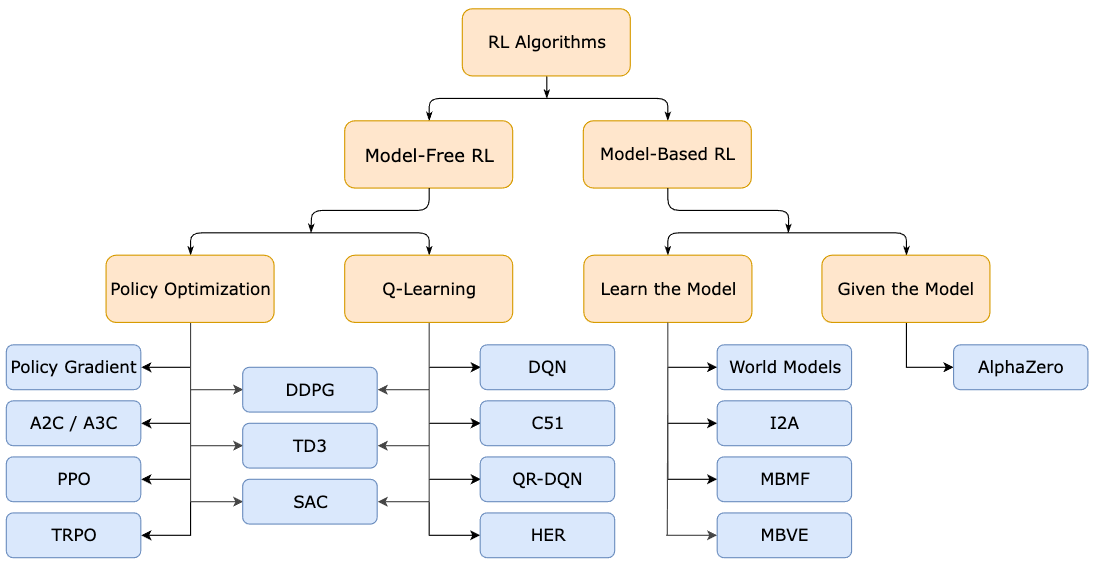
\includegraphics[width=13cm]{rl-taxonomy.png}
	\caption{A non-exhaustive taxonomy of RL algorithms. \cite{SpinningUp2018}.}
	\label{fig:rl-taxonomy}
\end{figure}


\subsection{Model-free vs model-based}

The first branching point in the \autoref{fig:rl-taxonomy} is whether the agent has access to a model  of the environment or needs to learn it.

Models are used for planning, meaning any way of deciding on a course of action by considering possible future situations before they are actually experienced. Methods for solving reinforcement learning problems that use models and planning are called model-based methods, as opposed to simpler model-free methods that are explicitly trial-and-error learners (viewed as almost the opposite of planning).

The advantages of having a model are that this allows the agent to plan by thinking ahead, seeing what would happen for a range of possible choices, and explicitly deciding between its options. A famouse example of this approach is AlphaZero \cite{silver2017mastering}.

Even if having a model could realy help the learner, a ground-truth model of the environment is usually not available to the agent. In this cases agents have to learn he model purely from experience, and the model-learning is fundamentally hard.

\subsection{What to learn}

Another critical branching point in an RL algorithm is deciding what to learn, this includes:
\begin{itemize}
	\item Policy
	\item Action-value function
	\item State-value function
	\item Model of the environment
\end{itemize}

Policy methods directly differentiate the objective function in \autoref{eq:objective}. In contrast, action-value function and state value function methods, estimate the the optimal state-function or Q-function of the optimal policy, but not explicitly the policy.


\subsection{Q-learning}


Q-Learning methods learn an approximator $Q_{\theta}(s,a)$ for the optimal action-value function, $Q^*(s,a)$. The Q-learning algorithm keeps an estimate $Q_t(s,a)$ of $Q^*(s,a)$ for each state-action pair $(s,a) \in S \times A$. Upon observing $(s_t, a_t, r_{t+1}, s_{t+1})$, the estimates are updated as follows \cite{series/synthesis/2010Szepesvari}:

\begin{equation}
	Q_{t+1}(s, a) = Q_t(s, a) + \alpha_t [\, r_{t+1} + \gamma \max_{a' \in A} Q_t(s_{t+1}, a') - Q_t(s_t, a_t)\,]
\end{equation}

$Q$ has been shown to converge with probability $1$ to $Q^*$ \cite{10.5555/3312046}. The Q-learning algorithm is shown below in procedural form.

\begin{algorithm}[H]
	\begin{algorithmic}
		\Require
		\Statex Learning rate $\alpha \in (0, 1]$
		\Procedure{QLearning}{$\mathcal{X}$, $A$, $R$, $T$, $\alpha$, $\gamma$}
		\State Initialize $Q(s,a)$, for all $s \in S$, $a \in A$, arbitrarly except that $Q(terminal, \cdot ) = 0$
		\While{$s$ is not terminal}
		\State Choose $a$ from $s$ using policy derived from $Q$
		\State Take action $a$, observe $r$, $s'$
		\State $Q(s, a) \gets Q(s, a) + \alpha [\cdot (r + \gamma  \max_{a} Q(s', a) - Q(s,a))]$
		\State $s \gets s'$
		%\Until{$S$ is terminal}
		\EndWhile
		\EndProcedure
	\end{algorithmic}
	\caption{Q-learning for estimating $\pi \approx \pi^*$}
	\label{alg:q-learning}
\end{algorithm}

In this case, the learned action-value function, $Q$, directly approximates $Q^*$, the optimal action-value function, independent of the policy being followed. Then from the lerned action-value function which aproximate $Q^*$ it's possible to derive $\pi^*$ by \autoref{eq:opt-policy}.

\subsection{Function aproximation}
Q-learning algorithm is a method to achieve optimal value functions and optimal policies. An agent that learns an optimal policy reaches his goal, but in practice this rarely happens. For the most intresting tasks, optimal policies can be generated only with extreme computational cost. Even if the agent have a complete and accurate model of the environment’s dynamics, it is usually not possible to simply compute an optimal policy by solving the Bellman optimality equation. A critical aspect of the problem facing the agent is always the computational power available to it, in particular, the amount of computation it can perform in a single time step.

The memory available is also an important constraint. A large amount of memory is often required to build up approximations of value functions, policies, and models. In the Q-learning algortihm(Algorithm \ref{alg:q-learning}.), it's necessary to build a table for each state-action pair, however, in many cases of practical interest there are far more states than could possibly be entries in a table, so this apporach is not scalable. In these cases the functions must be approximated, using some sort of more compact parameterized function representation.

Besides the space and time complexity when dealing with a huge number of states, it could be useful to achieve some approximations. For example, in approximating optimal behavior, there may be many states that the agent faces with such a low probability that selecting suboptimal actions for them has little impact on the amount of reward the agent receives. The online nature of reinforcement learning (i.e. data becomes available in a sequential order over time) makes it possible to approximate optimal policies in ways that put more effort into learning to make good decisions for frequently encountered states, at the expense of less effort for infrequently encountered states. This is one key property that distinguishes reinforcement learning from other approaches to approximately solving MDPs.

To make sensible decisions in large states space it is necessary to generalize from previous encounters states. Those previous encountered states are different from the current one but could be in some sense similar. The kind of generalization required is called function approximation because it takes examples from a desired function (e.g., a value function) and attempts to generalize from them to construct an approximation of the entire function. To achieve this, any of a broad range of existing methods for supervised-learning function approximation can be used simply by treating each update as a training example provided by interaction between the agent and the environment.

\subsection{ Deep RL}
Since achieveing generalization in state representation is simply function aproximation, artificial neural networks could be used to aproximate those functions. 
Most successful RL applications that deals with huge amount of stetes, relies on hand-crafted features combined with linear value functions or policy representations to aproximate state \cite{mnih2013atari}. The performance of such systems heavily relies on the quality of the feature representation.

In the work of David Silver et al. "Playing Atari with Deep Reinforcement Learning" \cite{mnih2013atari} they presented a deep learning model to successfully learn control policies directly from high-dimensional sensory input using reinforcement learning. The idea is to represent $Q(s,a)$ as a neural network  $f(s)$, which given a vector $s$ will output a vector of $Q$-values for all possible actions $a$.

In the work "Playing Atari with Deep Reinforcement Learning" \cite{mnih2013atari}, they developed an agent on the challenging domain of classic Atari 2600 games. They demonstrate that the deep Q-network agent, receiving only the pixels (processed by a convolutional neural network, hence a deep learning approach) and the game score as inputs, was able to surpass the performance of all previous algorithms and achieve a level comparable to that of a professional human games tester across a set of 49 games, using the same algorithm, network architecture and hyperparameters. This work bridges the divide between high-dimensional sensory inputs and actions, resulting in the first artificial agent that is capable of learning to excel at a diverse array of challenging tasks.

\begin{figure}[h]
	\centering
	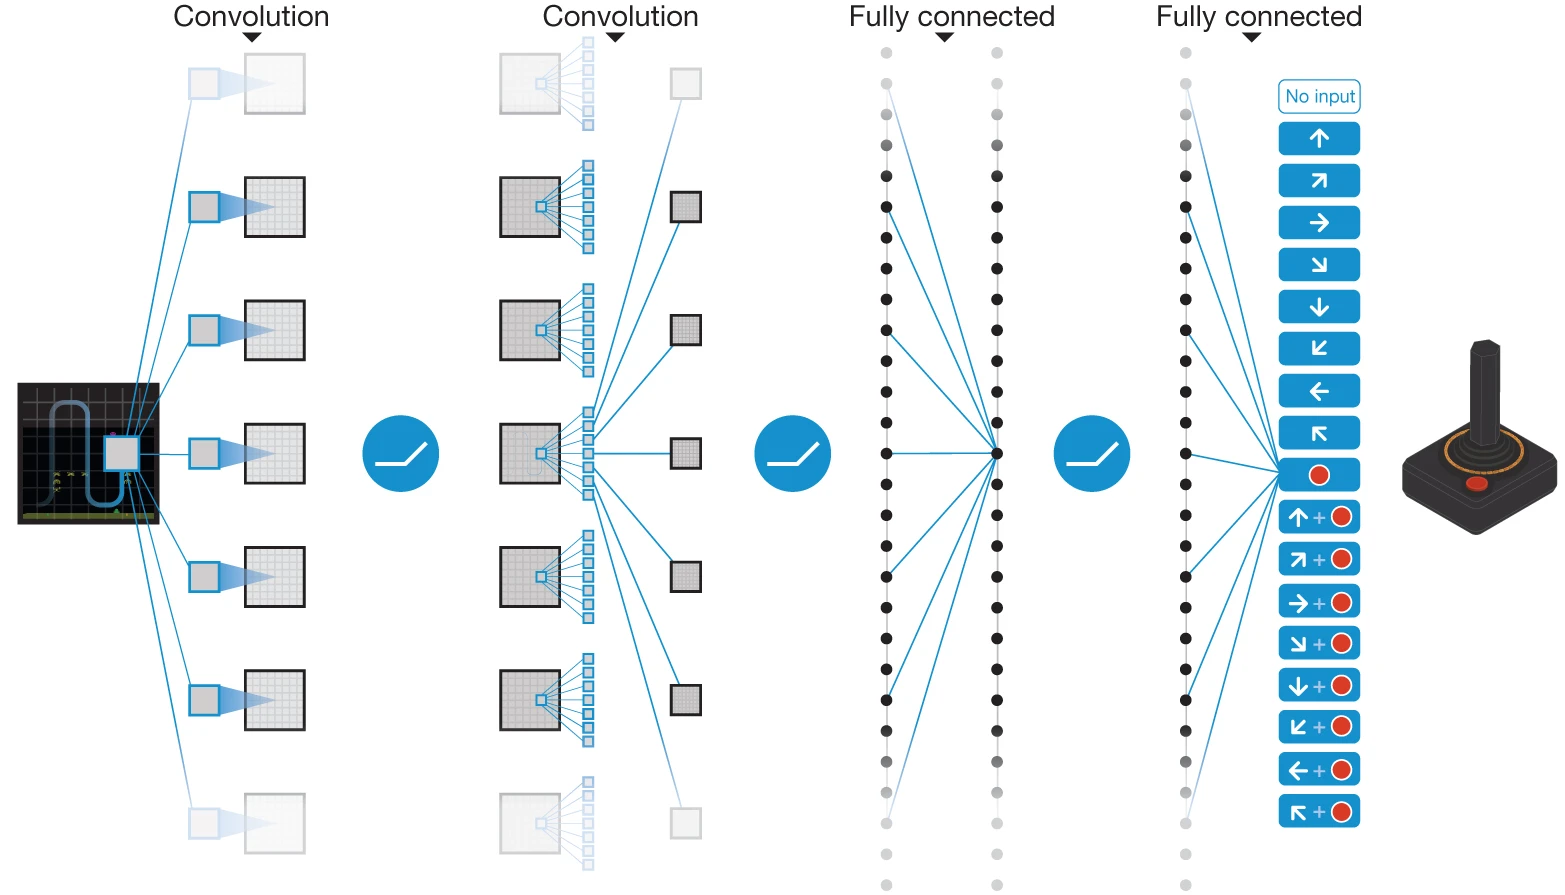
\includegraphics[width=14cm]{dqn-architecture.png}
	\caption{Architecure of the neural network used to predict actions. \cite{mnih2013atari}.}
	\label{fig:dqn-architecture.png}
\end{figure}



\section{Case study: AlphaGo zero}
\subsection{Motivation}
The game of Go has long been viewed as the most challenging of classic games for artificial intelligence owing to its enormous search space and the difficulty of evaluating board positions and moves. In the \autoref{tab:game-complexity} the complexity of some famous board games is summerized:


\begin{longtable}{|cccccc|}
	\hline
	\thead{ Game } &
	\thead{ Board size \\(positions) } &
	\thead{ State-space complexity\\ (as log to base 10) } &
	\thead{ Game-tree complexity \\(as log to base 10) } &
	\thead{ Ref. } &
	\thead{ Complexity class} \\
	\hline
	\hline
	Tic-tac-toe	& 9 & 3 & 5	& & PSPACE-complete[5] \\
	Connect Four & 42 & 13 & 21 & \cite{Allis1994SearchingFS} & in PSPACE \\
	Checkers & 32 & 20 or 18 & 40 & \cite{Allis1994SearchingFS} & EXPTIME-complete \cite{Robson1984NBN} \\
	Chess & 64 & 44 & 123 & \cite{doi:10.1080/14786445008521796} & EXPTIME-complete \cite{FRAENKEL1981199} \\
	Shogi & 81 & 71 & 226 & \cite{IIDA2002121} & EXPTIME-complete \cite{IIDA2002121}\\
	Go (19x19) & 361 & 170 & 360 & \cite{Allis1994SearchingFS} & EXPTIME-complete \cite{inproceedings} \\
	\hline
	
	
	\caption{Complexity of the most famous board game.}
	\label{tab:game-complexity}
	
	
\end{longtable}

As descriped in the work "Mastering the game of Go with deep neural networks and tree search"\cite{Silver_2016} by David Silver et al, all games of perfect information have an optimal value function, $v^*(s)$, which determines the outcome of the game, from every board position
or state $s$, under perfect play by all players. These games may be solved by recursively computing the optimal value function in a search tree
containing approximately $b^d$ possible sequences of moves, where $b$ is
the game’s breadth (number of legal moves per position) and $d$ is its depth (game length). In large games, such as chess ($b \approx 35$,$ d \approx 80$) \cite{Allis1994SearchingFS} and especially Go ( $b \approx 250$, $d \approx 150$) \cite{Allis1994SearchingFS}, exhaustive search is infeasible, but the effective search space can be reduced by two general principles. First, the depth of the search may be reduced by position evaluation: truncating the search tree at state $s$ and replacing the subtree below $s$ by an approximate value function $v(s) \approx v^*(s)$ that predicts the outcome from state $s$. This approach has led to superhuman performance in chess \cite{CAMPBELL200257} (the famous deep blue program that defeated Garry Kasparov) and checkers \cite{10.1007/3-540-48957-6_8} but it was believed to be intractable in Go due to the complexity of the game \cite{MULLER2002145}. Second, the breadth of the search
may be reduced by sampling actions from a policy $p(a|s)$ that is a probability distribution over possible moves $a$ in position $s$. For example,
Monte Carlo rollouts search to maximum depth without branching at all, by sampling long sequences of actions for both players from a
policy $p$. Averaging over such rollouts can provide an effective position evaluation, achieving weak amateur level play in Go \cite{Bouzy2004}.

\subsection{Versions  of AlphaGo}
In the first version of AlphaGo \cite{Silver_2016}, by a combination of supervised learning from human expert games, reinforcement learning from games of self-play and Monte Carlo simulation with value and policy networks, AlphaGo achieved a 99.8\% winning rate against other Go programs, and defeated the human European Go champion by 5 games to 0. That was the first time that a computer program has defeated a human professional player in the full-sized game of Go.

The next version of AlphaGo is AlphaGo Zero \cite{silver2017mastering}, an algorithm based solely on reinforcement learning, without human data, guidance or domain knowledge beyond game rules. Starting tabula rasa, AlphaGo Zero achieved superhuman performance in Go, winning 100–0 against the previously published, champion-defeating, AlphaGo.

\subsection{Neural network architecture  of AlphaGo Zero}
In AlphaGo Zero a depp neural $f_\theta$ with parameters $\theta$ is used. This neural network takes as an input the raw board representation $s$ of the position and outputs both move probabilities and a value, $f_\theta = (p,v)$. 

The output of the neural networks are:
\begin{itemize}
	\item Vector $p$: The vector of move probabilities $p$ represents the probability of selecting each move, $p_a = P(a | s)$
	\item Scalar $v$: The value $v$ is a scalar evaluation, estimating the probability of the current player winning from position $s$
\end{itemize}
In the previous version of AlphaGo \cite{Silver_2016}, two different deep neural networks were used to predict both $p$ and $v$. On the other hand, in AlphaGo Zero, these two neural networks are combined into a single one with two different outputs, treating the task as a multi-task learning problem. Another new aspect of these neural network is the introduction of many residual blocks of convolutional layers.

The final neural network takes as input features the board state $s$,  and consists in these layers:

\begin{enumerate}
	\item First convolutional block:
	\begin{enumerate}
		\item A convolution of 256 filters of kernel size 3 $\times$ 3 with stride 1
		\item Batch normalization
		\item A rectifier nonlinearity
	\end{enumerate}
	\item  39 residual blocks, each one applies the following modules sequentially to its input:
	\begin{enumerate}
		\item A convolution of 256 filters of kernel size 3 $\times$ 3 with stride 1
		\item Batch normalization
		\item A rectifier nonlinearity
		\item A convolution of 256 filters of kernel size 3 $\times$ 3 with stride 1
		\item Batch normalization
		\item A skip connection that adds the input to the block
		\item A rectifier nonlinearity
		The output of the residual tower is passed into two separate "heads" for computing the policy and value
	\end{enumerate}
	\item Two different "heads" for both policy and value
	\begin{itemize}
		\item The policy head:
		
		\begin{enumerate}
			\item A convolution of 2 filters of kernel size 1 $\times$ 1 with stride 1
			\item Batch normalization
			\item A rectifier nonlinearity
			\item A fully connected linear layer that outputs a vector of size $19^2 + 1 = 362$ ($19*19$ posible actions $+1$ for the pass acton)
		\end{enumerate}
		
		\item The value head:
		
		\begin{enumerate}
			\item A convolution of 1 filter of kernel size 1 $\times$ 1 with stride 1
			\item Batch normalization
			\item A rectifier nonlinearity
			\item A fully connected linear layer to a hidden layer of size 256
			\item A rectifier nonlinearity
			\item A fully connected linear layer to a scalar
			\item A tanh nonlinearity outputting a scalar in the range $[-1, 1]$ ($1$ representing the current player winning the game, $-1$ for the specular case)
		\end{enumerate}
	\end{itemize}
	
\end{enumerate}



\begin{figure}[H]
	\begin{subfigure}{.5\textwidth}
		\centering
		\includegraphics[height=6cm,trim={393px 313px 6855px 6134px},clip]{alpha_go_zero_cheat_sheet.png}
		\caption{The \textbf{convolutional layer.}}
		\label{fig:arch_convolution}
	\end{subfigure}
	\hfill
	\begin{subfigure}{.5\textwidth}
		\centering
		\includegraphics[height=11cm,trim={2518px 305px 4672px 4775px},clip]{alpha_go_zero_cheat_sheet.png}
		\caption{A \textbf{residual layer.}}
		\label{fig:arch_residual}
	\end{subfigure}
	\newline
	\begin{subfigure}{0.5\textwidth}
		\centering
		\includegraphics[height=10cm,trim={380px 1665px 6840px 3798px},clip]{alpha_go_zero_cheat_sheet.png}
		\caption{The \textbf{value head.}}
		\label{fig:arch_value}
	\end{subfigure}
	\hfill
	\begin{subfigure}{0.5\textwidth}
		\centering
		\includegraphics[height=8cm,trim={2567px 2995px 4688px 3197px},clip]{alpha_go_zero_cheat_sheet.png}
	\caption{The \textbf{policy head.}}
	\label{fig:arch_policy}
	\end{subfigure}
\end{figure}


\begin{figure}[H]\ContinuedFloat
	\begin{subfigure}{1\textwidth}
		\centering
		\includegraphics[height=16cm,angle=90,trim={1600px 243px 5916px 3678px},clip]{alpha_go_zero_cheat_sheet.png}
		\caption{\textbf{Full neural network.}}
		\label{fig:arch_full}
	\end{subfigure}
	\caption[Caption for LOF]{The architecture of AlphaGo Zero. Diagram from this article.\footnotemark}
\end{figure}

\footnotetext{\url{https://medium.com/applied-data-science/alphago-zero-explained-in-one-diagram-365f5abf67e0}}

\subsection{Reinforcement learning in AlphaGo Zero}
The neural network in AlphaGo Zero is trained from games of self­ play by a novel reinforcement learning algorithm. In each position $s$, an MCTS search is executed, guided by the neural network $f_\theta$. The MCTS search outputs probabilities $\pi$ of playing each move. These search probabilities usually select much stronger moves than the raw move probabilities $p$ of the neural network $f_\theta(s)$; MCTS may therefore be viewed as a powerful policy improvement operator. Self­play with search may be viewed as a powerful policy evaluation operator. During the self-play the MCTS-based policy is used to select each move, and the game winner $z$ is used as a sample of the value $v$ (the winning player).

\subsubsection{Self-play}

The main idea of this reinforcement learning algorithm is to use these search operators in a policy iteration procedure: the neural network’s parameters are updated to make the move probabilities and value $(p, v) = f_\theta(s)$ more closely match the improved search probabilities and self play winner $(\pi, z)$; these new parameters are used in the next iteration of self-play to make the search even stronger.

The self-play pipeline is performed as following (see \autoref{fig:alpha-zero-self_play}): The program plays a game $s_1, \, ..., \, s_t$ against itself. In each position $s_t$, an MCTS $\alpha_\theta$ is executed (see \autoref{fig:alpha-zero-mcts}) using the latest neural network $f_\theta$. Moves are selected according to the search probabilities computed by the MCTS, $a_t \sim \pi_t$. The terminal position $s_T$ is scored according to the rules of the game to compute the game winner $z$.

\begin{figure}[H]
		\centering
		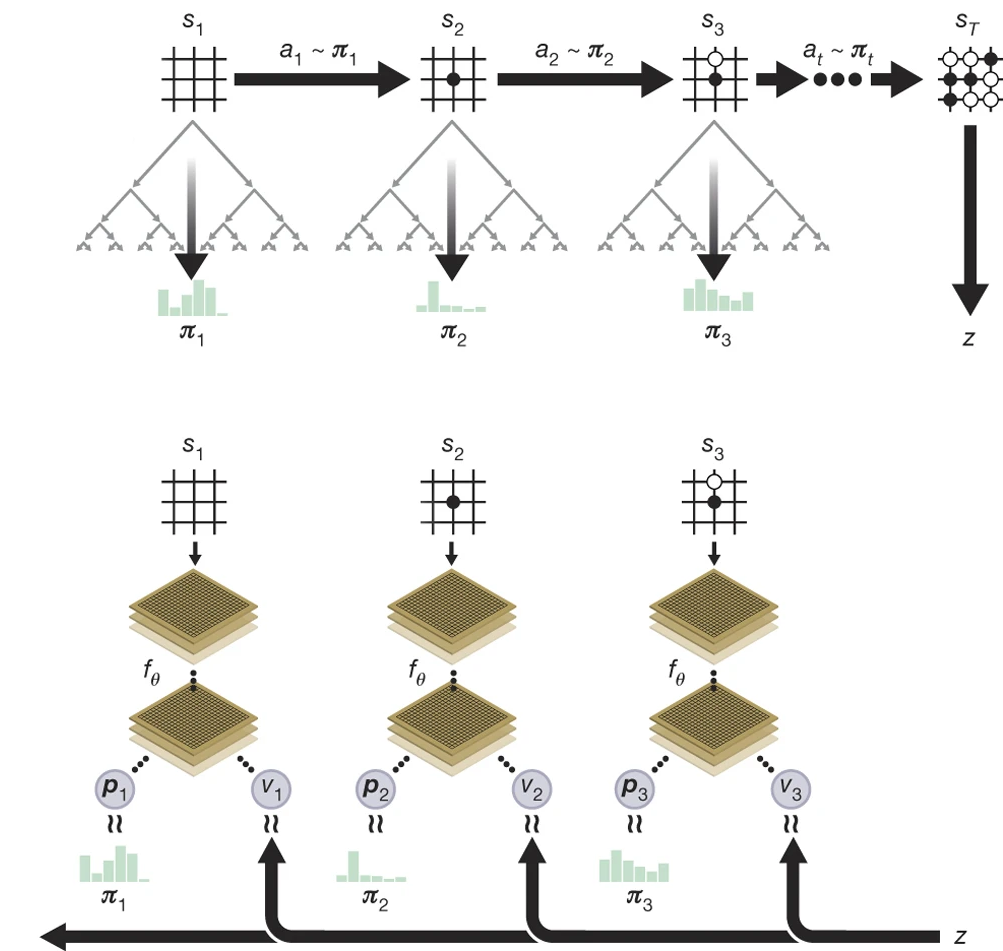
\includegraphics[width=12cm,trim={66px 430px 0px 0px},clip]{alpha_go_zero_training.png}
		
		\caption{
			\textbf{Self-play} AlphaGo Zero.\cite{Silver_2016}}
		\label{fig:alpha-zero-self_play}
\end{figure}

During the self-play procedure, each tuple $(s_t, \pi_t, z)$ is stored as a training example for the training phase. During the training, the neural network takes the raw board position $s_t$ as input, passes it through many convolutional layers with parameters $\theta$, and outputs both a vector $p_t$, representing a probability distribution over moves, and a scalar value $v_t$, representing the probability of the current player winning in position $s_t$ (see \autoref{fig:alpha-zero-mcts}). The neural network parameters $\theta$ are updated to maximize the similarity of the policy vector $p_t$ to the search probabilities $\pi_t$, and to minimize the error between the predicted winner $v_t$ and the game winner $z$ (see \autoref{eq:loss_function_alphazero}). The new parameters are used in the next iteration of self-play as shown in \autoref{fig:alpha-zero-self_play}.

\begin{figure}[H]
	\centering
	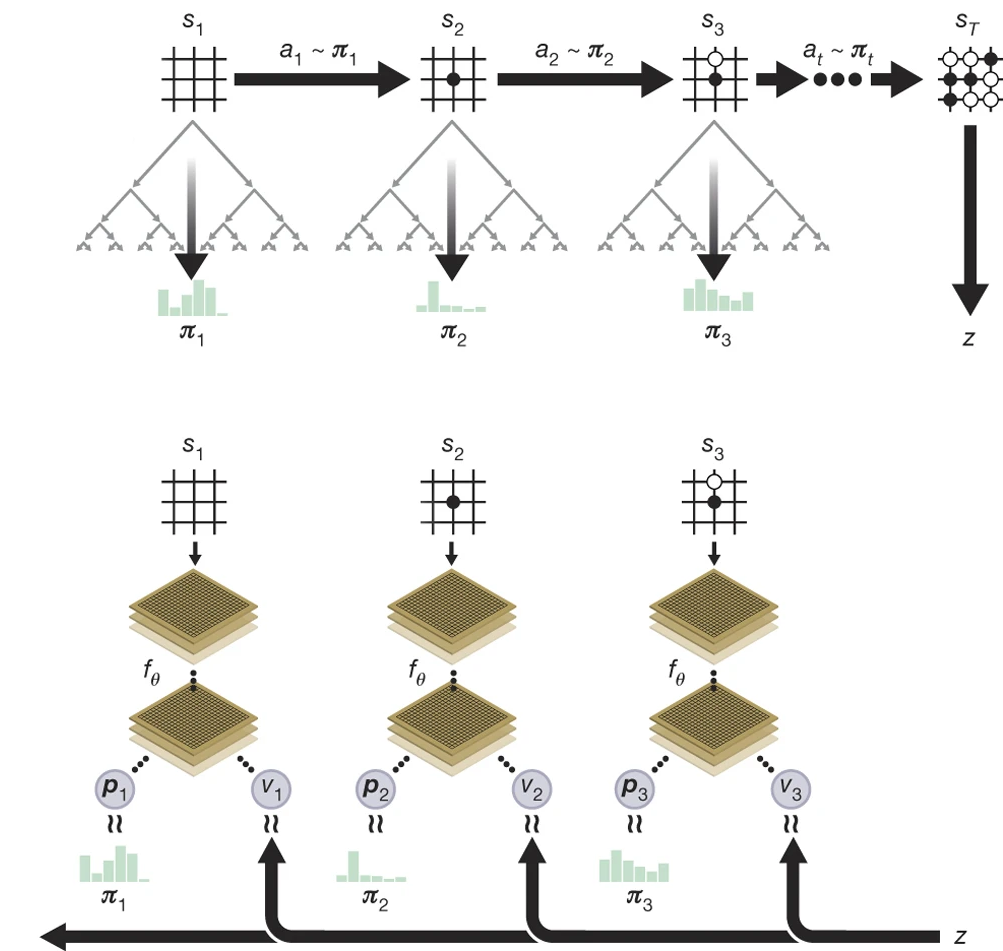
\includegraphics[width=12cm,trim={0px 0px 0px 280px},clip]{alpha_go_zero_training.png}
	
	\caption{\textbf{Neural network training} in AlphaGo Zero.\cite{Silver_2016}}
\end{figure}


\subsubsection{MCTS}
The MCTS uses the neural network $f_\theta$ to guide its simulations (see \autoref{fig:alpha-zero-mcts}). Each edge $(s, a)$ in the search tree stores a prior probability $P(s, a) = p_\theta(a | s)$, a visit count $N(s, a)$, and an action-value $Q(s, a)$. 

Each simulation starts from the root state and iteratively selects moves $a_t  = \argmax_a{Q(s_t,a) + U(s_t,a)}$, until a leaf node $s'$ is encountered. This leaf position is expanded and evaluated only once by the network to generate both prior probabilities and evaluation, $(P(s', \cdot), \, V(s')) = f_\theta(s')$.

The action-value function is defined as:
\begin{equation}
	Q(s_t, a) = \frac{1}{N(s,a)} \sum_{s'\, | \, s,\, a \rightarrow s'}{V(s')}
\end{equation}
where $s, a \rightarrow s'$ indicates that a simulation eventually reached $s'$ after taking move a from position $s$.

The reason why the chosen action $a$ maximise the sum $Q(s_t,a) + U(s_t,a)$ and not only the action-value function $Q(s_t, a)$ is because $U(s_t,a)$ acts as an exploration factor. The exploration-exploitation tradeoff is taken into account by this factor $U(s_t,a)$, which is defined as:
\begin{equation}
	U(s, a) = c_{puct}P(s, a)\frac{\sum_b N(s,b)}{1+N(s,a)}
\end{equation}
where $c_{puct}$ is a constant determining the level of exploration; this search control strategy initially prefers actions with high prior probability and low visit count, but asympotically prefers actions with high action value.

MCTS may be viewed as a self-play algorithm that, given neural network parameters $\theta$ and a root position $s$, computes a vector of search probabilities recommending moves to play, $\pi = \alpha_\theta(s)$.

The key points of the algorithm are summarized in the \autoref{fig:alpha-zero-mcts}, where is possible to see how each simulation traverses the tree of the MCTS by selecting the edge with maximum action value $Q$, plus an upper confidence bound $U$ that depends on a stored prior probability $P$ and visit count $N$ for that edge (which is incremented once traversed).
\begin{figure}[H]
	\centerline{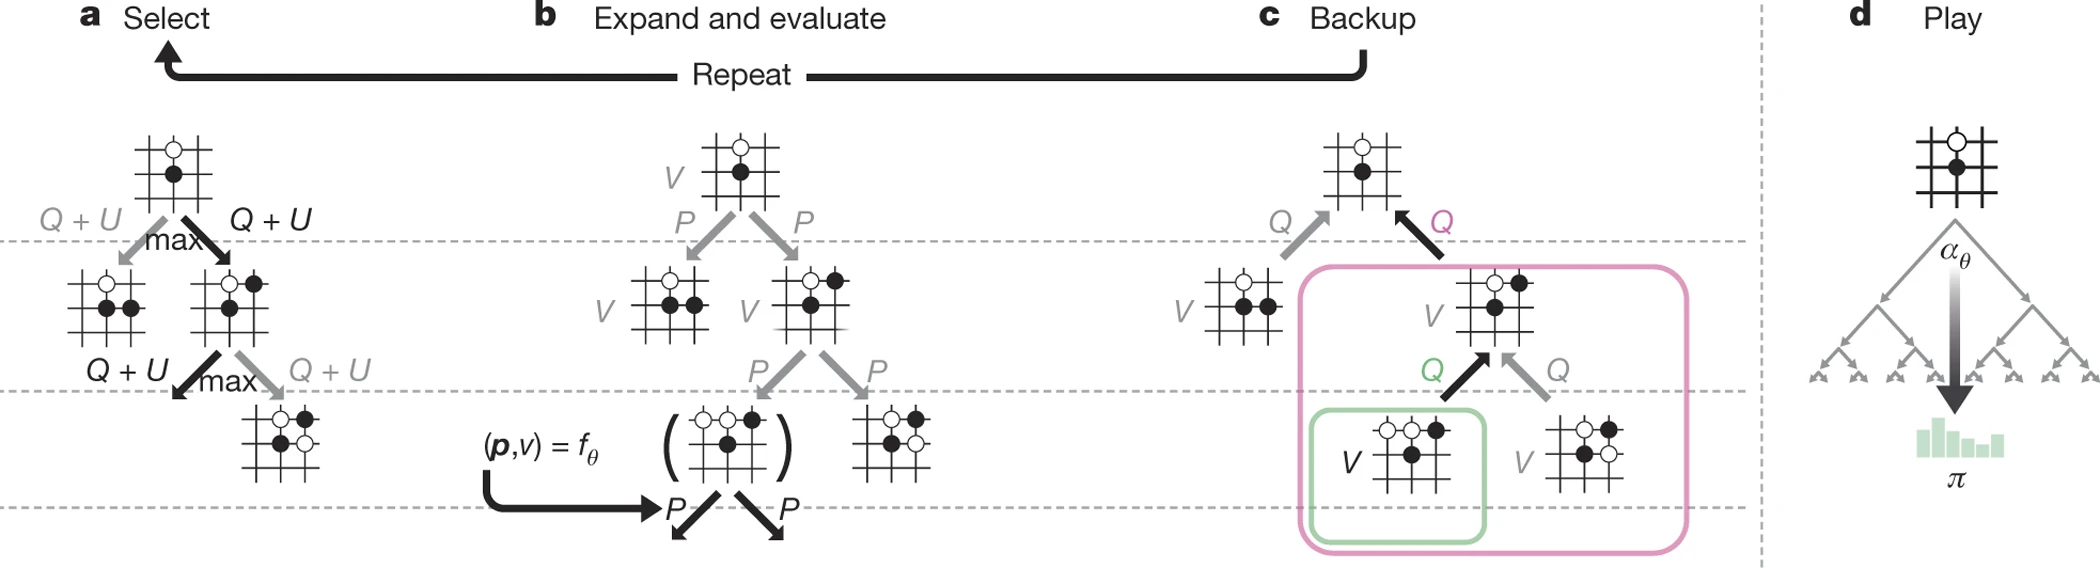
\includegraphics[width=15cm]{alpha-zero-mcts.png}}
	\caption{\textbf{MCTS procedure} in AlphaGo Zero\cite{Silver_2016}:\\ \textbf{(a)} Each simulation traverses the tree by selecting the edge with maximum action value $Q$, plus an upper confidence bound $U$ that depends on a stored prior probability $P$ and visit count $N$ for that edge (which is incremented once traversed).\\ \textbf{(b)} The leaf node is expanded and the associated position $s$ is evaluated by the neural network $(P(s', \cdot), \, V(s')) = f_\theta(s')$; the vector of $P$ values are stored in the outgoing edges from $s$.\\ \textbf{(c)} Action-value $Q$ is updated to track the mean of all evaluations $V$ in the subtree below that action.\\ \textbf{(d)} Once the search is complete, search probabilities $\pi$ are returned.}
	\label{fig:alpha-zero-mcts}
\end{figure}

\subsubsection{Loss function}
The parameters $\theta$ are adjusted by gradient descent on a loss function $L$ that sums over the mean-squared error to (to have $v$ as close as possible to $z$) and cross-entropy losses (to have $p$ as close as possible to $\pi$), respectively:
\begin{equation}\label{eq:loss_function_alphazero}
	(p,v) = f_\theta(s),\, L = (z-v)^2 - \pi_t log(p) + c \norm{\theta}^2
\end{equation}
where $c$ is a parameter controlling the level of L2 weight regularization to prevent overfitting.

\section{Hands on: Connect4 zero}
Ho aggiunto parallelizazione come in DQN

No residual blocks dato che la rete ho meno risorse

\bibliographystyle{unsrt}  % TODO: Change style
\bibliography{references}

\end{document}
